%% Creator: Inkscape inkscape 0.91, www.inkscape.org
%% PDF/EPS/PS + LaTeX output extension by Johan Engelen, 2010
%% Accompanies image file 'figures/reactors_wibench.pdf' (pdf, eps, ps)
%%
%% To include the image in your LaTeX document, write
%%   \input{<filename>.pdf_tex}
%%  instead of
%%   \includegraphics{<filename>.pdf}
%% To scale the image, write
%%   \def\svgwidth{<desired width>}
%%   \input{<filename>.pdf_tex}
%%  instead of
%%   \includegraphics[width=<desired width>]{<filename>.pdf}
%%
%% Images with a different path to the parent latex file can
%% be accessed with the `import' package (which may need to be
%% installed) using
%%   \usepackage{import}
%% in the preamble, and then including the image with
%%   \import{<path to file>}{<filename>.pdf_tex}
%% Alternatively, one can specify
%%   \graphicspath{{<path to file>/}}
%% 
%% For more information, please see info/svg-inkscape on CTAN:
%%   http://tug.ctan.org/tex-archive/info/svg-inkscape
%%
\begingroup%
  \makeatletter%
  \providecommand\color[2][]{%
    \errmessage{(Inkscape) Color is used for the text in Inkscape, but the package 'color.sty' is not loaded}%
    \renewcommand\color[2][]{}%
  }%
  \providecommand\transparent[1]{%
    \errmessage{(Inkscape) Transparency is used (non-zero) for the text in Inkscape, but the package 'transparent.sty' is not loaded}%
    \renewcommand\transparent[1]{}%
  }%
  \providecommand\rotatebox[2]{#2}%
  \ifx\svgwidth\undefined%
    \setlength{\unitlength}{563.89536526bp}%
    \ifx\svgscale\undefined%
      \relax%
    \else%
      \setlength{\unitlength}{\unitlength * \real{\svgscale}}%
    \fi%
  \else%
    \setlength{\unitlength}{\svgwidth}%
  \fi%
  \global\let\svgwidth\undefined%
  \global\let\svgscale\undefined%
  \makeatother%
  \begin{picture}(1,0.65267091)%
    \put(0,0){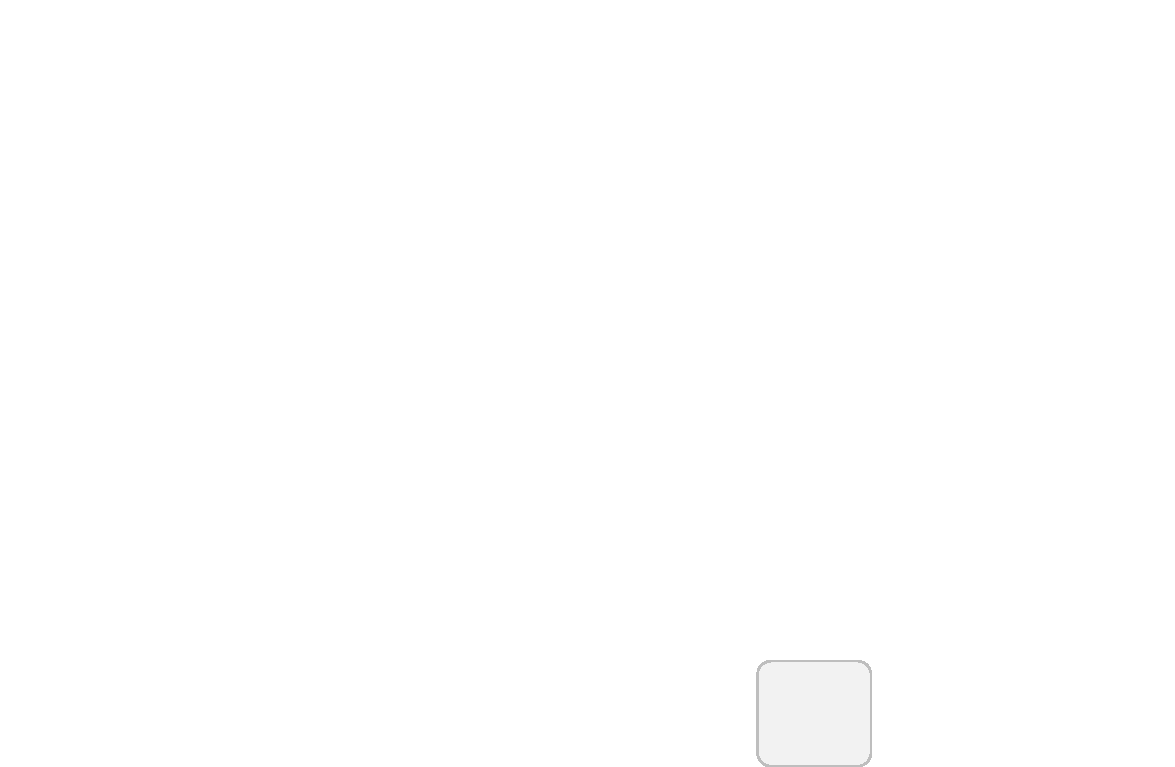
\includegraphics[width=\unitlength,page=1]{figures/reactors_wibench.pdf}}%
    \put(0.6526984,0.08228477){\color[rgb]{0,0,0}\makebox(0,0)[lb]{\smash{WiBench}}}%
    \put(0,0){\includegraphics[width=\unitlength,page=2]{figures/reactors_wibench.pdf}}%
    \put(0.01844314,0.6441587){\color[rgb]{0,0,0}\makebox(0,0)[lb]{\smash{GenerateInputs}}}%
    \put(0,0){\includegraphics[width=\unitlength,page=3]{figures/reactors_wibench.pdf}}%
    \put(0.00851222,0.51221933){\color[rgb]{0,0,0}\makebox(0,0)[lb]{\smash{(0, 1nsec)}}}%
    \put(0,0){\includegraphics[width=\unitlength,page=4]{figures/reactors_wibench.pdf}}%
    \put(0.13193937,0.55265236){\color[rgb]{0,0,0}\makebox(0,0)[lb]{\smash{\textbf{2}}}}%
    \put(0,0){\includegraphics[width=\unitlength,page=5]{figures/reactors_wibench.pdf}}%
    \put(0.13193937,0.60798177){\color[rgb]{0,0,0}\makebox(0,0)[lb]{\smash{\textbf{1}}}}%
    \put(0,0){\includegraphics[width=\unitlength,page=6]{figures/reactors_wibench.pdf}}%
    \put(0.23834209,0.58882928){\color[rgb]{0,0,0}\makebox(0,0)[lb]{\smash{Encoder}}}%
    \put(0,0){\includegraphics[width=\unitlength,page=7]{figures/reactors_wibench.pdf}}%
    \put(0.37892474,0.58882928){\color[rgb]{0,0,0}\makebox(0,0)[lb]{\smash{RateMatcher}}}%
    \put(0,0){\includegraphics[width=\unitlength,page=8]{figures/reactors_wibench.pdf}}%
    \put(0.55976562,0.58882928){\color[rgb]{0,0,0}\makebox(0,0)[lb]{\smash{Scrambler}}}%
    \put(0,0){\includegraphics[width=\unitlength,page=9]{figures/reactors_wibench.pdf}}%
    \put(0.71919299,0.58882928){\color[rgb]{0,0,0}\makebox(0,0)[lb]{\smash{Modulator}}}%
    \put(0,0){\includegraphics[width=\unitlength,page=10]{figures/reactors_wibench.pdf}}%
    \put(0.87927356,0.58845893){\color[rgb]{0,0,0}\makebox(0,0)[lb]{\smash{Precoder}}}%
    \put(0,0){\includegraphics[width=\unitlength,page=11]{figures/reactors_wibench.pdf}}%
    \put(0.04585149,0.41390658){\color[rgb]{0,0,0}\makebox(0,0)[lb]{\smash{SubCarrierMapper}}}%
    \put(0,0){\includegraphics[width=\unitlength,page=12]{figures/reactors_wibench.pdf}}%
    \put(0.26561509,0.41390658){\color[rgb]{0,0,0}\makebox(0,0)[lb]{\smash{SCFDMAModulator}}}%
    \put(0,0){\includegraphics[width=\unitlength,page=13]{figures/reactors_wibench.pdf}}%
    \put(0.5015007,0.41390658){\color[rgb]{0,0,0}\makebox(0,0)[lb]{\smash{ChannelReactor}}}%
    \put(0,0){\includegraphics[width=\unitlength,page=14]{figures/reactors_wibench.pdf}}%
    \put(0.70909382,0.41336561){\color[rgb]{0,0,0}\makebox(0,0)[lb]{\smash{SCFDMADemodulator}}}%
    \put(0,0){\includegraphics[width=\unitlength,page=15]{figures/reactors_wibench.pdf}}%
    \put(0.03746624,0.23781008){\color[rgb]{0,0,0}\makebox(0,0)[lb]{\smash{SubCarrierDemapper}}}%
    \put(0,0){\includegraphics[width=\unitlength,page=16]{figures/reactors_wibench.pdf}}%
    \put(0.28833335,0.23781008){\color[rgb]{0,0,0}\makebox(0,0)[lb]{\smash{EqualizerReactor}}}%
    \put(0,0){\includegraphics[width=\unitlength,page=17]{figures/reactors_wibench.pdf}}%
    \put(0.50868771,0.23781008){\color[rgb]{0,0,0}\makebox(0,0)[lb]{\smash{TransformDecoderReactor}}}%
    \put(0,0){\includegraphics[width=\unitlength,page=18]{figures/reactors_wibench.pdf}}%
    \put(0.80658014,0.23781008){\color[rgb]{0,0,0}\makebox(0,0)[lb]{\smash{Demodulator}}}%
    \put(0,0){\includegraphics[width=\unitlength,page=19]{figures/reactors_wibench.pdf}}%
    \put(0.03547694,0.08228477){\color[rgb]{0,0,0}\makebox(0,0)[lb]{\smash{Descrambler}}}%
    \put(0,0){\includegraphics[width=\unitlength,page=20]{figures/reactors_wibench.pdf}}%
    \put(0.23559506,0.08228477){\color[rgb]{0,0,0}\makebox(0,0)[lb]{\smash{RxRateMatcher}}}%
    \put(0,0){\includegraphics[width=\unitlength,page=21]{figures/reactors_wibench.pdf}}%
    \put(0.45130415,0.08228477){\color[rgb]{0,0,0}\makebox(0,0)[lb]{\smash{TurboDecoder}}}%
    \put(0,0){\includegraphics[width=\unitlength,page=22]{figures/reactors_wibench.pdf}}%
  \end{picture}%
\endgroup%
